\documentclass[journal, onecolumn, final, letterpaper, 11pt]{IEEEtran}
\usepackage{setspace}

\usepackage{cite}
\usepackage{amsmath}
\usepackage{mathtools}
\usepackage{svg}
\usepackage{epstopdf}
\usepackage{float}
\usepackage{cmap}
\usepackage{wrapfig}
\usepackage[font=footnotesize, center]{caption}

\font\myfont=cmr12 at 18pt

\begin{spacing}{1.0}
\title{\myfont{\textmd{A Scalable Dynamic Capacitive Wireless Power Transfer System Architecture}}}
\normalsize
\end{spacing}

\begin{document}
\maketitle
 
\doublespacing

\vspace{-0.85cm}
\begin{spacing}{1.4}
\noindent \textbf{{\small Abstract}} -- \small{This digest presents a novel power-scalable architecture for dynamic capacitive wireless power transfer (WPT) systems utilizing an active variable reactance (AVR) rectifier. The AVR rectifier enables continuous compensation, allowing the WPT system to maintain high-efficiency power transfer at a fixed frequency by appropriately distributing power between its two branches. A transformer-based power-splitting method is used to realize a scalable AVR rectifier while maintaining high system efficiency and wide dynamic compensation range. Furthermore, a state-space model of this architecture is developed and used to design a full state feedback controller. To validate the proposed approach, a 6.78 MHz 12-kW dynamic capacitive WPT system is built. Three 4-kW full-bridge inverters and three half-bridge rectifiers per AVR branch are paralleled to achieve this power level. The system's operation is demonstrated through both simulations and experiments on the hardware prototype.}
\end{spacing}

\vspace{-0.15cm}

\section{Introduction}

Wireless power transfer (WPT) is becoming increasingly important and has the potential to accelerate the widespread adoption of electric vehicles (EVs), especially amongst vehicles that routinely travel along fixed routes such as buses and warehouse forklifts. Capacitive WPT systems can be lighter, cheaper, and smaller than comparable inductive WPT systems due to the absence of ferrite cores. The ability of capacitive WPT systems to transfer high power at high efficiency has been demonstrated, thus proving the viability of this technology \cite{2025_Etta_APEC}.

One main challenge of WPT systems is the extreme sensitivity to the value of the coupling capacitance or mutual inductance between the receiver and the transmitter. The recently proposed active variable reactance (AVR) rectifier addresses these challenges and efficiently provides variable compensation in high-frequency WPT systems \cite{2019_Sinha_Journal}. Additionally, a novel time-domain solution for the control of the AVR rectifier has been proposed in \cite{2025_Liao_COMPEL} and demonstrated on hardware at low power. This approach allows an AVR-equipped capacitive WPT system to dynamically compensate for changes in the coupling capacitance automatically.

Capacitive WPT systems typically operate at multi-MHz frequencies, which pose another significant challenge for high-power operation due to limitations in commercially available GaN devices. Various power-combining approaches have been proposed in \cite{2022_Surakitbovorn_Journal, 2025_Etta_APEC}, with the transformer-based power-combining and power-splitting approach in \cite{2025_Etta_APEC} being particularly effective due to its scalability, low component count, and simple implementation. This digest combines the AVR rectifier architecture \cite{2019_Sinha_Journal} with the transformer-based power-splitting method \cite{2025_Etta_APEC} to obtain a scalable dynamic capacitive WPT system.

In this digest, an AVR-equipped scalable dynamic capacitive WPT system architecture is proposed. A state-space model is developed for this architecture, and a full-state-feedback controller is designed using the proposed model to automatically compensate for variations in coupling capacitance. Finally, the proposed architecture and controller are validated first in simulation, then on a prototype 6.78 MHz, 12-kW dynamic capacitive WPT hardware system. 

\begin{figure*}[!ht]
	\centering
	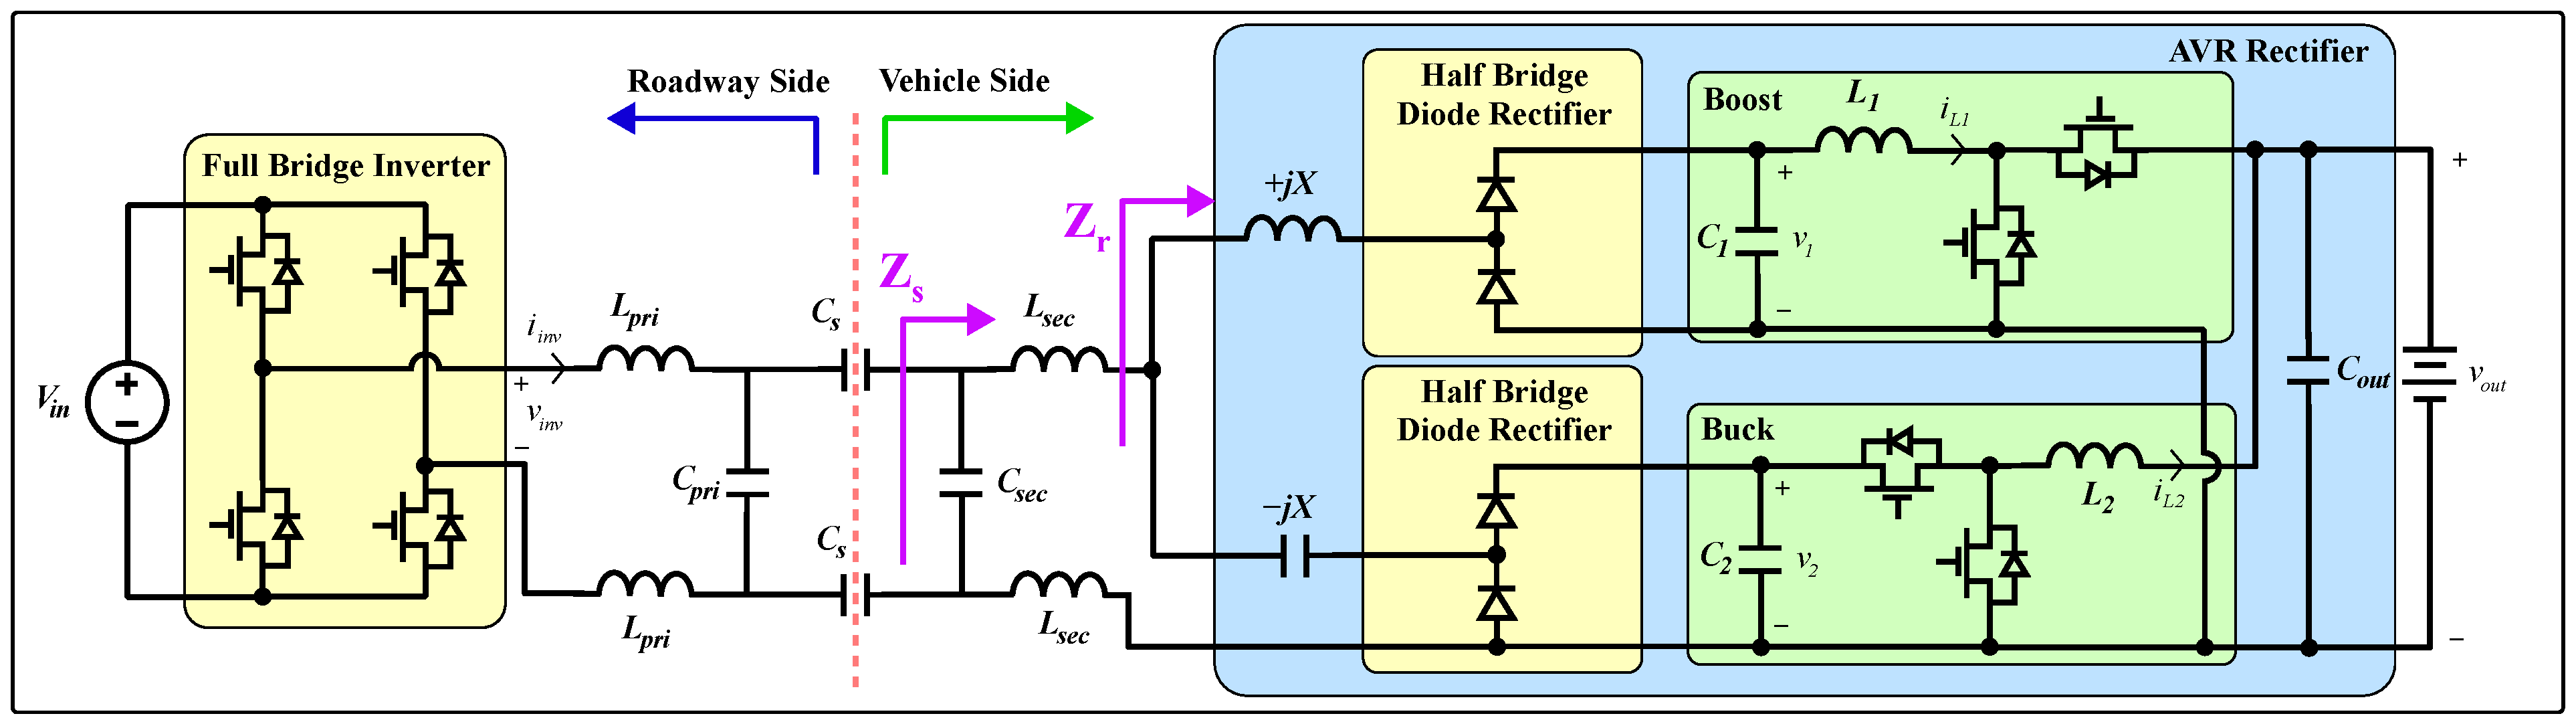
\includegraphics[width=\textwidth]{figures/wpt_with_avr_full_schematic_eps.eps}
	\caption{Dynamic capacitive wireless power transfer system with active variable reactance rectifier schematic.}
	\label{fig:original_full_schematic}
	
	\vspace{-0.5cm}
\end{figure*}

\section{Dynamic Capacitive Wireless Power Transfer System with an AVR Rectifier}
\label{sec:system}

Figure \ref{fig:original_full_schematic} presents the practical circuit schematic of the dynamic capacitive WPT system with the AVR rectifier. A DC input bus is connected to a full-bridge inverter. $C_s$ is the coupling capacitance between the roadway-side and vehicle-side coupling plates. The L-section matching network ($L_{pri}$, $C_{pri}$, $L_{sec}$, $C_{sec}$) surrounding $C_s$ is designed to provide a voltage gain to minimize displacement current through the air gap while compensating the reactance of $C_s$ such that the loading on the inverter is near-resistive, allowing the inverter to achieve soft-switching.

The AVR rectifier has two branches: a top branch containing a boost converter attached to an inductive reactance $+jX$ through a half-bridge rectifier, and a bottom branch containing a buck converter attached to a capacitive reactance $-jX$ through a half-bridge rectifier. By independently varying the amount of power processed in each branch, the AVR rectifier can maintain the desired constant output power ($P_{out})$ while compensating for coupling variations by modulating the impedance seen at the input of the AVR rectifier ($z_r$). Throughout this digest, the following notation is used: $p_{out}$ is the time-varying measured variable, $P_{out}$ is the constant nominal DC value, and $\hat{p}_{out}$ is the small-signal variable. They are related as $p_{out}(t) \equiv P_{out} + \hat{p}_{out}(t)$. 

Equations \ref{eqn:pout}-\ref{eqn:zsec} give $p_{out}$, $z_r$, and $z_s$ as a function of the large-signal circuit states as labeled in Fig. \ref{fig:original_full_schematic}:

\footnotesize
\vspace{-0.8cm}
\begin{subequations}\label{eqn:pout_zin}
	\begin{align}
		p_{out} &= p_1 + p_2 = v_1 i_{L1} + v_{out} i_{L2} \label{eqn:pout} \\
		z_r &= \operatorname{Re}(z_r) + j\cdot\operatorname{Im}(z_r) = r_r + jx_r = \frac{k_{rec}^2 v_1^2 v_2^2 + v_1v_{out}i_{L1}i_{L2}X^2}{k_{rec}(v_1v_2^2i_{L1} + v_{out}v_1^2i_{L2})} + jX\frac{v_1 i_{L1}v_2^2 - v_{out} i_{L2}v_1^2}{v_1 i_{L1}v_2^2 + v_{out} i_{L2}v_1^2} \label{eqn:zin} \\
		z_s &=  \operatorname{Re}(z_s) + j\cdot\operatorname{Im}(z_s) = r_s + jx_s = \frac{r_r}{(1-\omega_s C_{sec} x_r)^2 + (\omega_s C_{sec}r_r)^2} + j\Bigl[\omega_s L_{sec} + \frac{x_r - \omega_s C_{sec} (r_r^2 + x_r^2)}{(1-\omega_s C_{sec} x_r)^2 + (\omega_s C_{sec}r_r)^2}\Bigr] \label{eqn:zsec}
	\end{align}
\end{subequations}
\normalsize

\vspace{-0.2cm}

$k_{rec}$ is a gain associated with the half-bridge rectifiers under sinusoidal approximation, $X$ is the differential reactance $\pm jX$ attached to the two branches, and $\omega_s$ is the inverter switching frequency in rad/s. When the coupling capacitance $C_s$ changes by an amount $\Delta C_s$, Eqns. \ref{eqn:pout}-\ref{eqn:zsec} are utilized to adjust the operation of the AVR rectifier such that the real part of the impedance looking into the secondary $Z_s$ is held constant at its nominal value $r_s = R_s$. This also guarantees $p_{out} = P_{out}$, as well as resistive loading on the inverter. A derivation of Eqn. \ref{eqn:zin} can be found in \cite{2019_Sinha_Journal}; a derivation of Eqn. \ref{eqn:zsec} will be provided in the full paper.

\begin{figure*}[!t]
\vspace{-0.5cm}
	\centering
	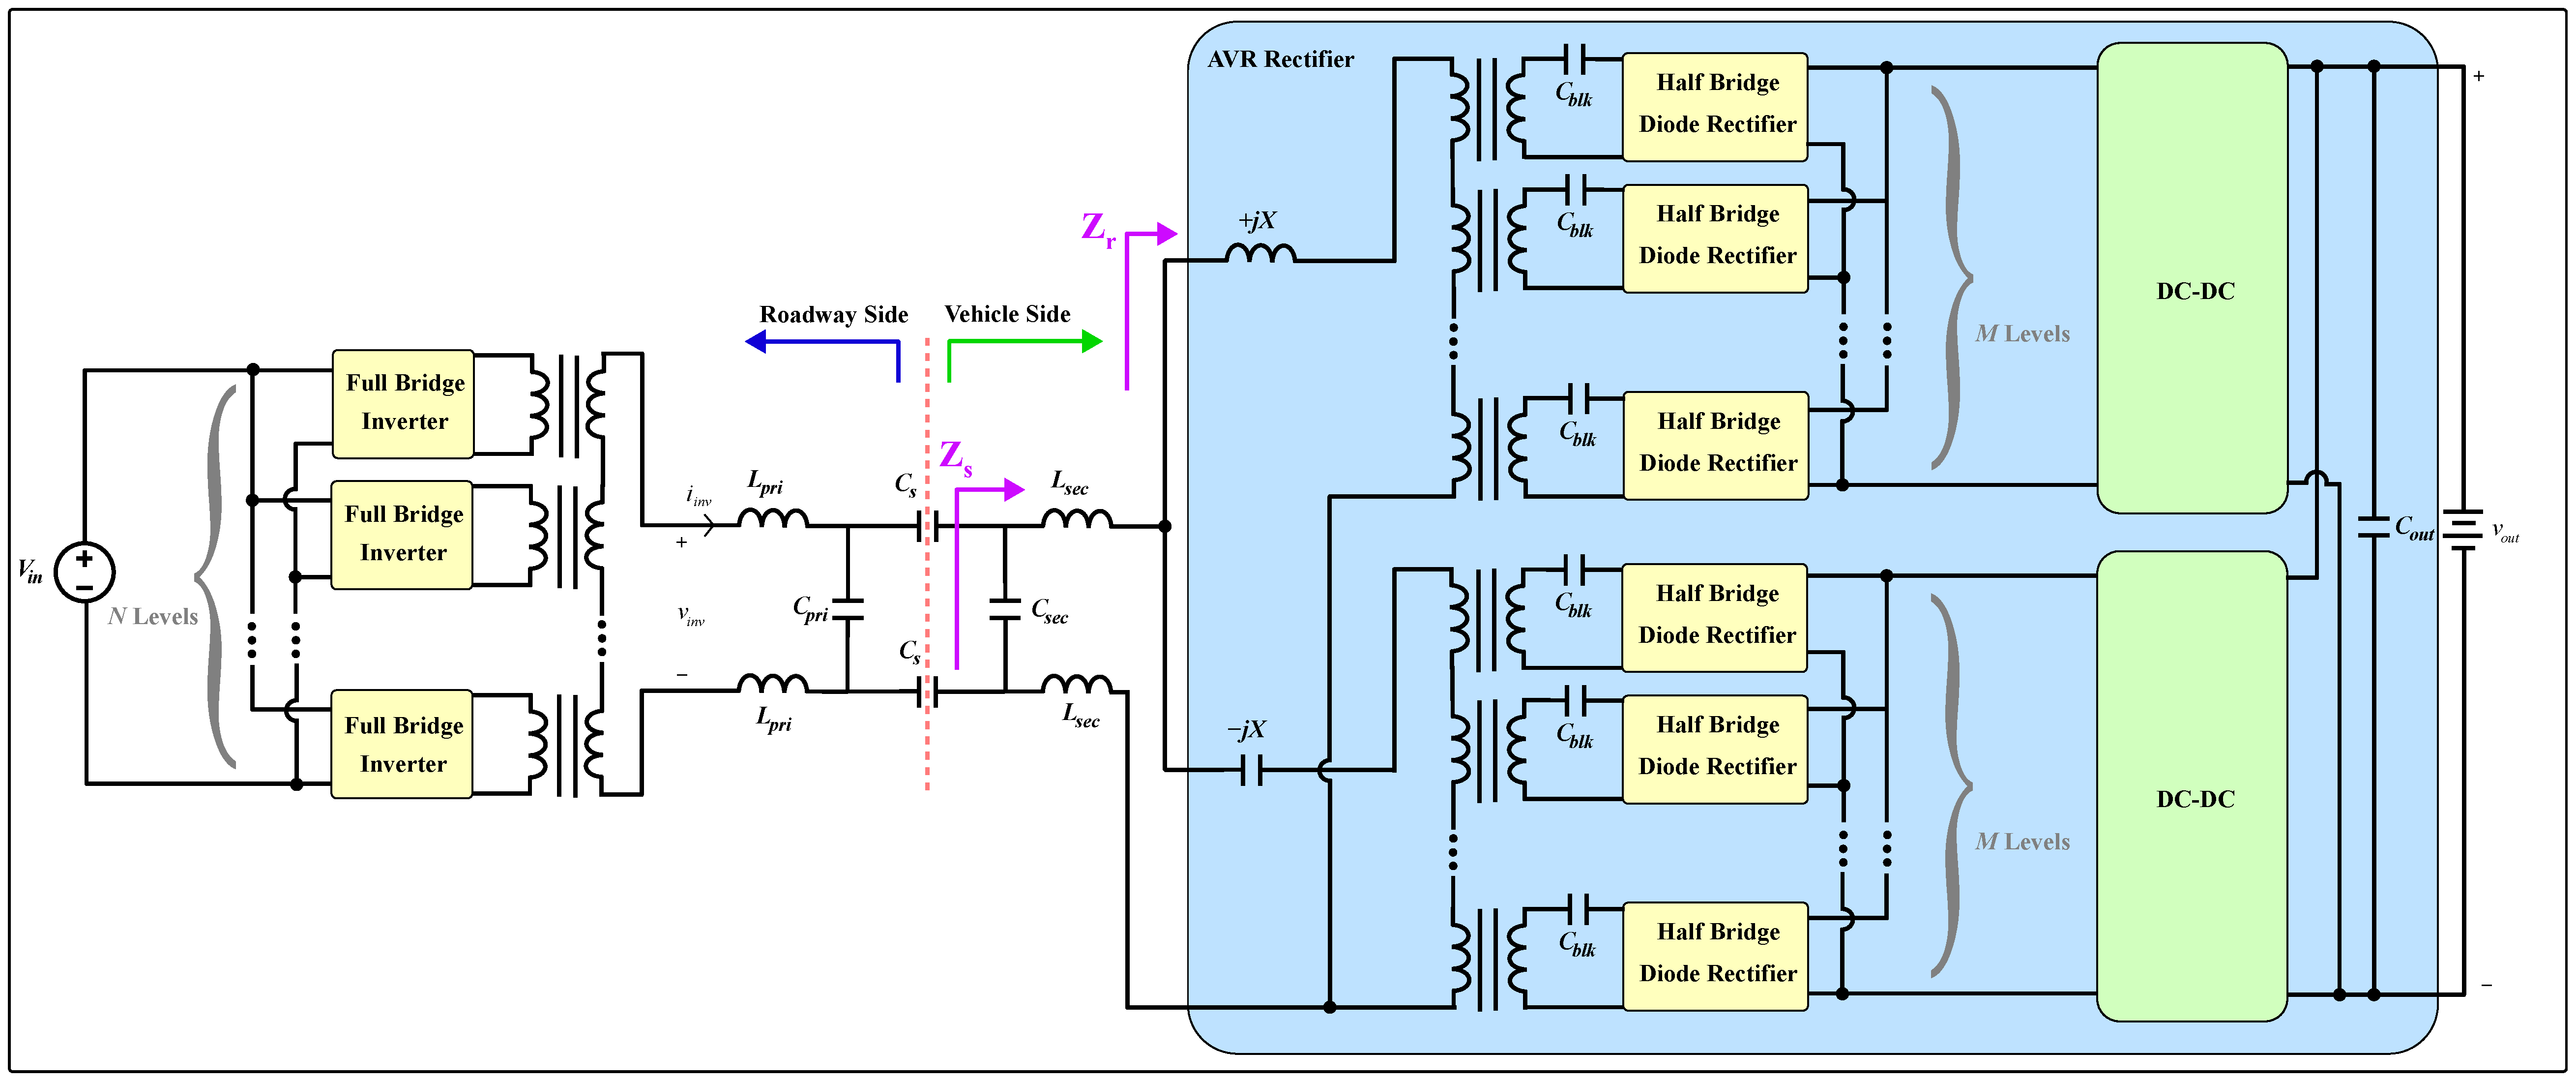
\includegraphics[width=\textwidth]{figures/scalable_wpt_with_avr_full_schematic_eps.eps}
	\caption{Proposed scalable dynamic capacitive wireless power transfer system schematic. All transformers have a 1:1 turns ratio.}
	\label{fig:scalable_full_schematic}
	
	\vspace{-0.5cm}
\end{figure*}

\section{Scalable Architecture for Dynamic Capacitive WPT}
\label{sec:scalable}

This section motivates and presents a novel topology for scaling the capacitive WPT system described in Section \ref{sec:system} to higher powers while maintaining dynamic compensation capability. In high-power capacitive WPT systems, the performance bottleneck is typically at the high-frequency inverters, as the GaN FETs used have much lower power-handling capabilities compared to the SiC Schottky diodes and switches in the rectifiers and DC-DC converters. To address inverter power scaling issues, multiple inverters can be paralleled using transformers as described in \cite{2025_Etta_APEC}. But, the performance bottleneck of the system is now shifted to the SiC diodes in the high frequency half-bridge rectifiers in the AVR rectifier. Additionally, there is an inherent tradeoff between the efficiency of the matching network, the gain of the matching network, and the AVR rectifier's compensation range. Thus, having a large current gain while achieving a target matching network efficiency causes the maximum compensation range of the resulting AVR rectifier to be prohibitively narrow, decreasing the utility of the system. \cite{2019_Sinha_Journal} To meet the growing power demands of EV chargers without compromising the dynamic compensation range of WPT systems, there is a need to develop power-scaling methods that enable effective parallel operation of the AVR rectifier.

Figure \ref{fig:scalable_full_schematic} shows the proposed novel scalable dynamic capacitive WPT topology. On the roadway side, an $N$-level stacked-inverter architecture introduced in \cite{2025_Etta_APEC} combines the power from $N$ high-frequency inverters at the input. On the vehicle side, power is split between the $+jX$ and $-jX$ branches. On each branch, an $M$-level stacked-rectifier structure using a series-in parallel-out transformer splits the power into $M$ high-frequency half-bridge diode rectifiers. The rectified power is then combined in parallel and fed through a single DC-DC converter on each branch. This topology meshes the wide dynamic compensation range of the AVR rectifier with the high-efficiency scalable system proposed in \cite{2025_Etta_APEC}, all with a low component count. This novel architecture is the first significant contribution of this digest.

\section{Modeling, Control, and Simulation of the Scalable Dynamic Capacitive WPT System}
\label{sec:mod_ctrl_sim}

\begin{figure}[t]
\vspace{-0.4 cm}
\centering
\begin{minipage}{.5\textwidth}
  \centering
  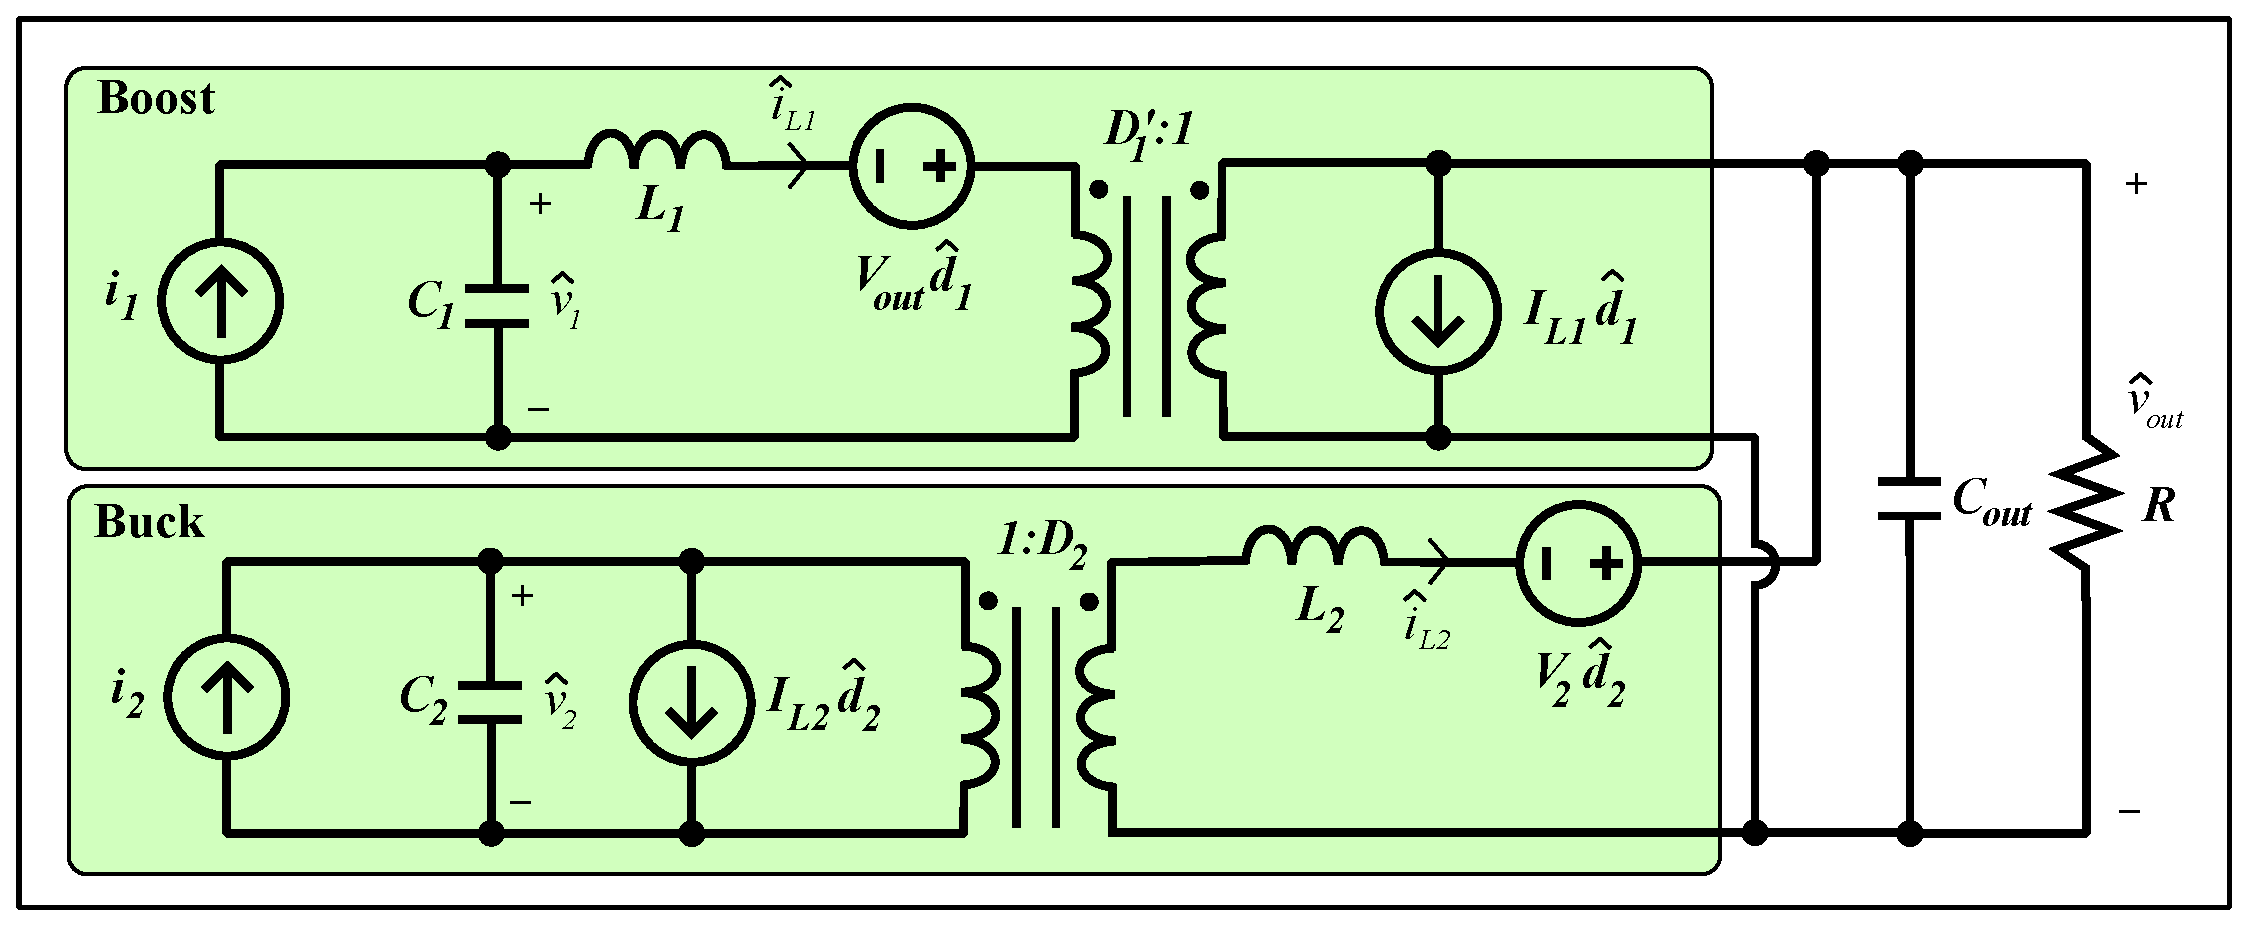
\includegraphics[width=\linewidth]{figures/avr_ss_model_schematic_eps.eps}
  \caption{Schematic of the linearized small-signal model of the AVR rectifier.}
  \label{fig:small_signal}
\end{minipage}%
\begin{minipage}{.5\textwidth}
  \centering
  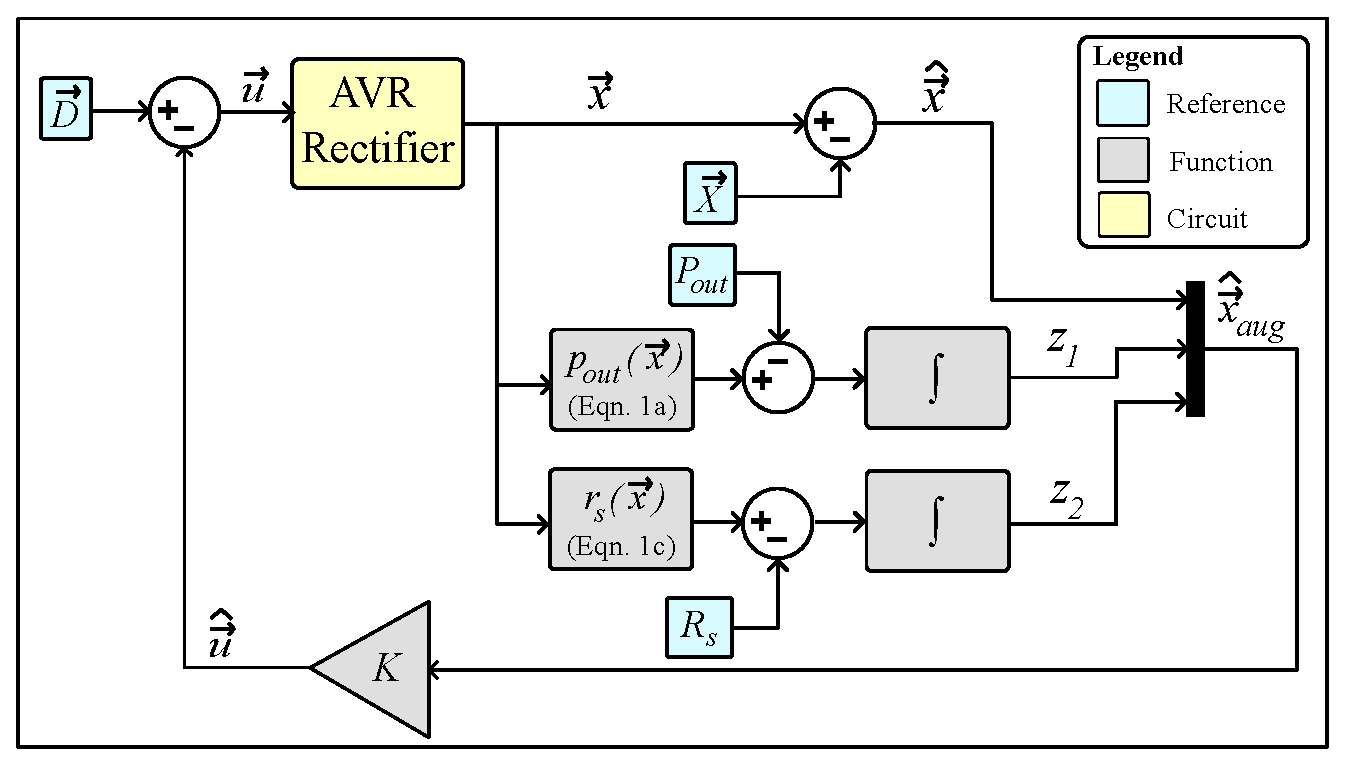
\includegraphics[width=0.95\linewidth]{figures/block_diagram_eps.eps}
  \caption{Block diagram of the state-space control loop. $p_{out}(\vec{x})$ and $r_s(\vec{x})$ are given by Eqns. \ref{eqn:pout} and \ref{eqn:zsec}. $\vec{D}$ contains nominal duties of the buck and boost converters.}
  \label{fig:block_diagram}
\end{minipage}
\vspace{-0.4cm}
\end{figure}

\begin{figure*}[!b]
	\centering
	\vspace{-0.5cm}
	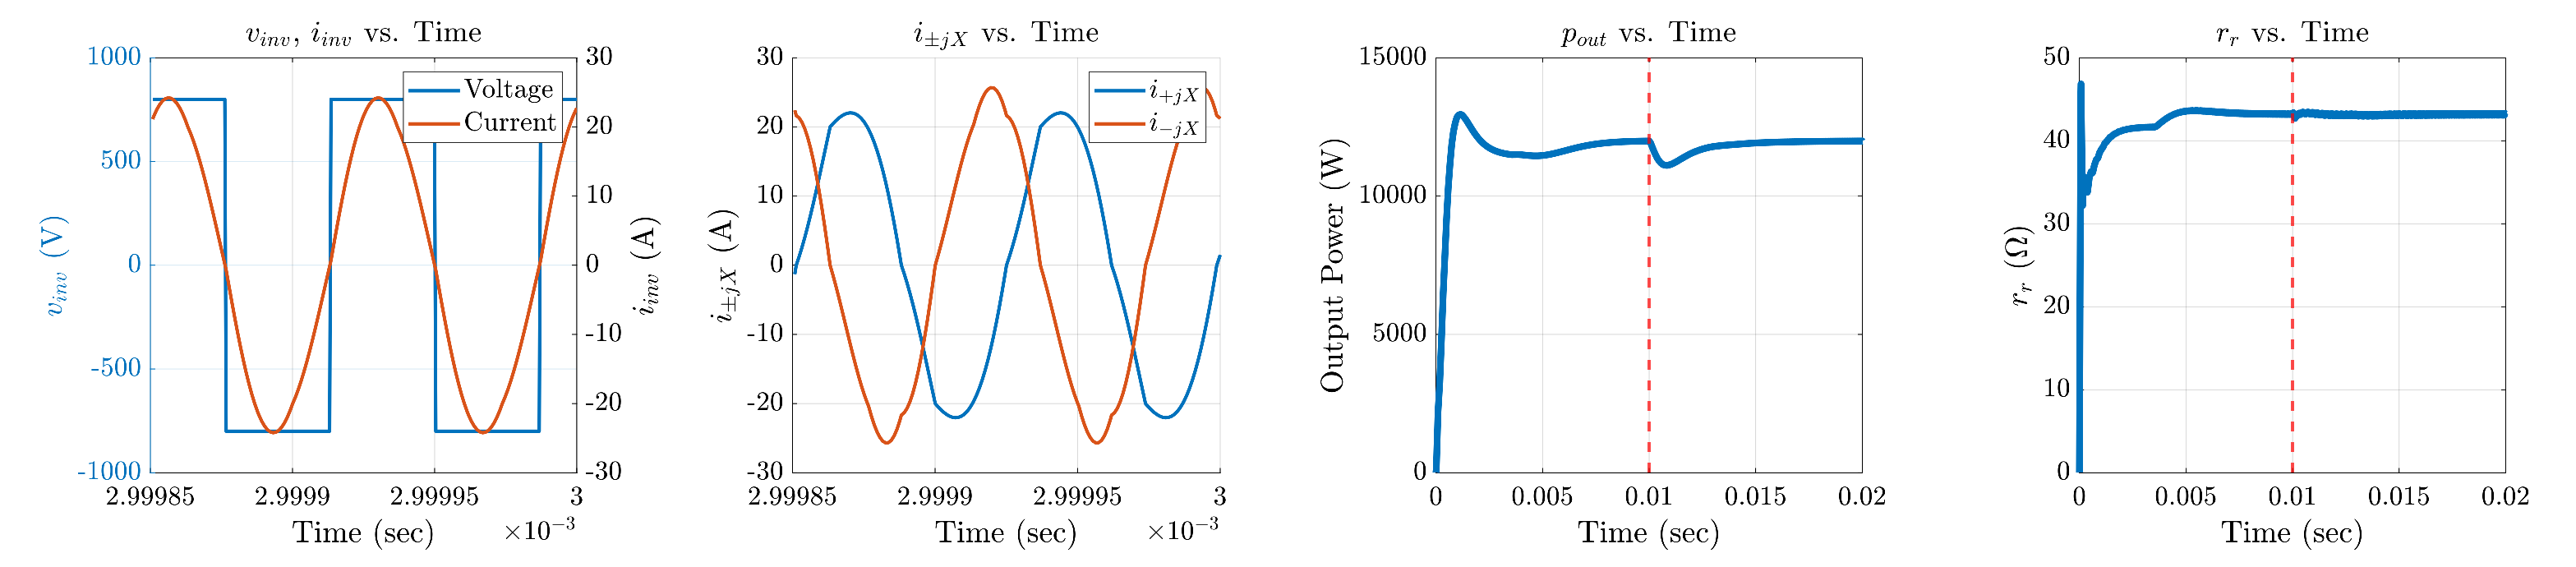
\includegraphics[width=\textwidth]{figures/sim_results_eps.eps}
	\caption{From left to right: inverter output waveforms $v_{inv}$ and $i_{inv}$ in steady-state; AVR branch currents $i_{+jX}$ and $i_{-jX}$ in steady-state; $p_{out}$ and $r_r$ vs. time, showing the AVR rectifier's startup transient under the proposed controller for $t \in [0, 0.01)$, followed by a step change in coupling reactance $\Delta X_s$ at time $t = 0.01$, marked by the red vertical line.}
	\label{fig:sim_results}
\end{figure*}

In this section, a model for the scalable WPT architecture is developed in state space using methods presented in \cite{2025_Liao_COMPEL, 2010_Mayo_CONIELECOMP}. A full state feedback controller is then designed utilizing this model to provide dynamic compensation for a changing coupling capacitance. Finally, the proposed topology and controller are validated in simulation. Since the proposed architecture of Fig. \ref{fig:scalable_full_schematic} does not modify the small-signal schematic of the AVR rectifier (Fig. \ref{fig:small_signal}), the derivation of the state-space model presented in \cite{2025_Liao_COMPEL} applies nearly exactly. Deviations occur only in the value of $k_{rec}$ and the partial derivatives of $z_r$, which now become the partial deriviatives of $z_s$, taken using Eqn. \ref{eqn:zsec}. The resulting augmented state-space model is given by Eqn. \ref{eqn:aug_ss_model}; a full derivation of the updated state-space model will be presented in the full paper. A full state feedback controller is designed using methods employed in \cite{2025_Liao_COMPEL, 2007_Williams}. Figure \ref{fig:block_diagram} shows the complete block diagram of the system under closed-loop control.

A model is built in Simulink and PLECS to validate the proposed topology and controller for a 6.78 MHz, 12-kW system with $V_{in} = V_{out} = 400$ V. Figure \ref{fig:sim_results} shows steady-state inverter output waveforms and AVR branch currents. It also shows the control objectives $p_{out}$ and $r_s$ being controlled to $P_{out} = 12 \text{ kW}$ and $R_s = 43.2 \text{ }\Omega$, while the coupling reactance is disturbed by an amount $\Delta X_s \equiv \frac{1}{2 \pi f_s}(\frac{1}{C_{s,nom}} - \frac{1}{C_s})$, where $f_s$ is the switching frequency, and $C_{s,nom}$ is the nominal coupling capacitance. The state-space model, full state feedback controller, and simulation validation of the proposed architecture comprise the second significant contribution of this digest.

\scriptsize
\begin{equation}
\label{eqn:aug_ss_model}
\frac{d}{dt}
\begin{bmatrix}
	\hat{v}_{out} \\
	\hat{v}_1 \\
	\hat{v}_2 \\
	\hat{i}_{L1} \\
	\hat{i}_{L2} \\
	z_1 \\
	z_2
\end{bmatrix}
=
\begin{bmatrix}
	-\frac{1}{RC_{out}} & 0 & 0 & \frac{D_1'}{C_{out}} & \frac{1}{C_{out}} & 0 & 0 \\
	0 & 0 & 0 & -\frac{1}{C_1} & 0 & 0 & 0 \\
	0 & 0 & 0 & 0 & -\frac{D_2}{C_2} & 0 & 0\\
	-\frac{D_1'}{L_1} & \frac{1}{L_1} & 0 & 0 & 0 & 0 & 0 \\
	-\frac{1}{L_2} & 0 & \frac{D_2}{L_2} & 0 & 0 & 0 & 0 \\
	-I_{L2} & -I_{L1} & 0 & -V_1 & -V_{out} & 0 & 0 \\
	-\frac{\partial r_s}{\partial v_{out}} & -\frac{\partial r_s}{\partial v_{1}} & -\frac{\partial r_s}{\partial v_{2}} & -\frac{\partial r_s}{\partial i_{L1}} & -\frac{\partial r_s}{\partial i_{L2}} & 0 & 0
\end{bmatrix}
\begin{bmatrix}
	\hat{v}_{out} \\
	\hat{v}_1 \\
	\hat{v}_2 \\
	\hat{i}_{L1} \\
	\hat{i}_{L2} \\
	z_1 \\
	z_2
\end{bmatrix}
+
\begin{bmatrix}
	-\frac{I_{L1}}{C_{out}} & 0 \\
	0 & 0 \\
	0 & -\frac{I_{L2}}{C_2} \\
	\frac{V_{out}}{L_1} & 0 \\
	0 & \frac{V_2}{L_2} \\
	0 & 0 \\
	0 & 0
\end{bmatrix}
\begin{bmatrix}
	\hat{d}_1 \\
	\hat{d}_2
\end{bmatrix}
\end{equation}
\normalsize

\begin{figure}[!b]
\vspace{-0.6cm}
\centering
\begin{minipage}{0.5\textwidth}
  \centering
  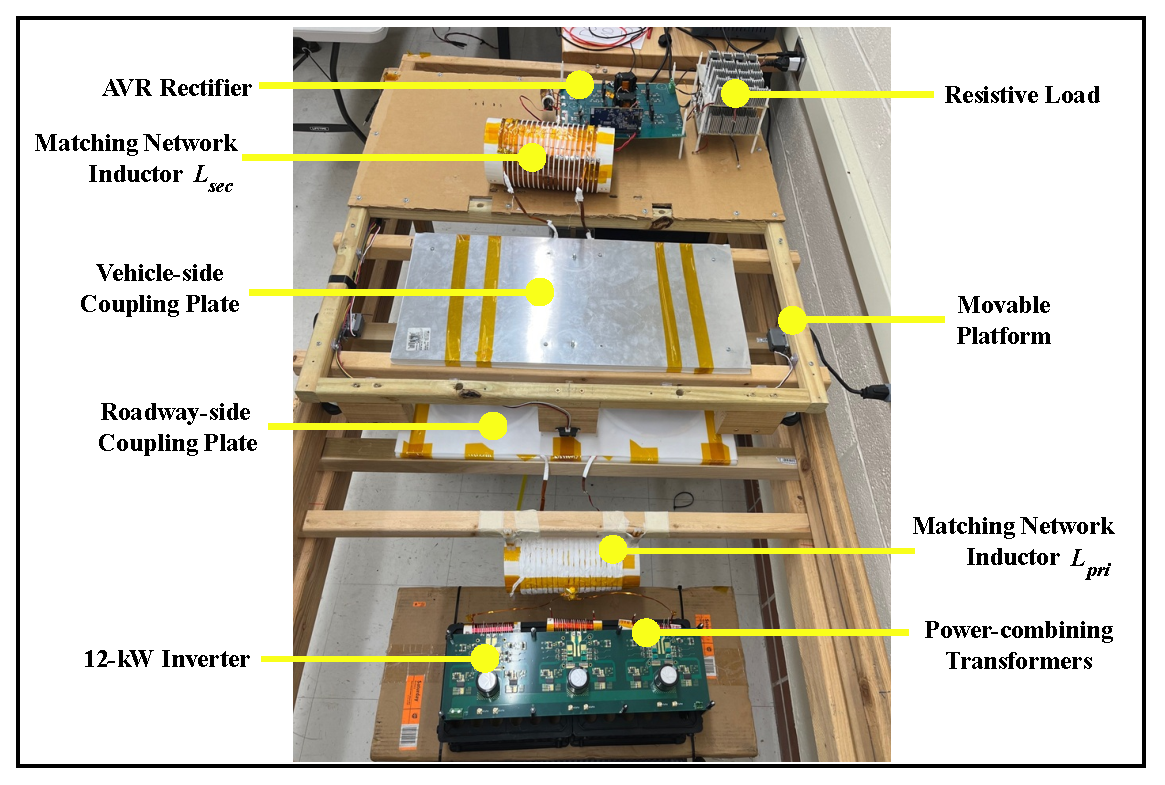
\includegraphics[width=0.9\textwidth]{figures/hardware_pic_annotated_eps.eps}
	\caption{Annotated photograph of the hardware prototype. A load resistor $R$ is used in place of a battery.}
  \label{fig:hardware_prototype}
\end{minipage}%
\hspace{0.5cm}
\begin{minipage}{0.45\textwidth}
  \centering
  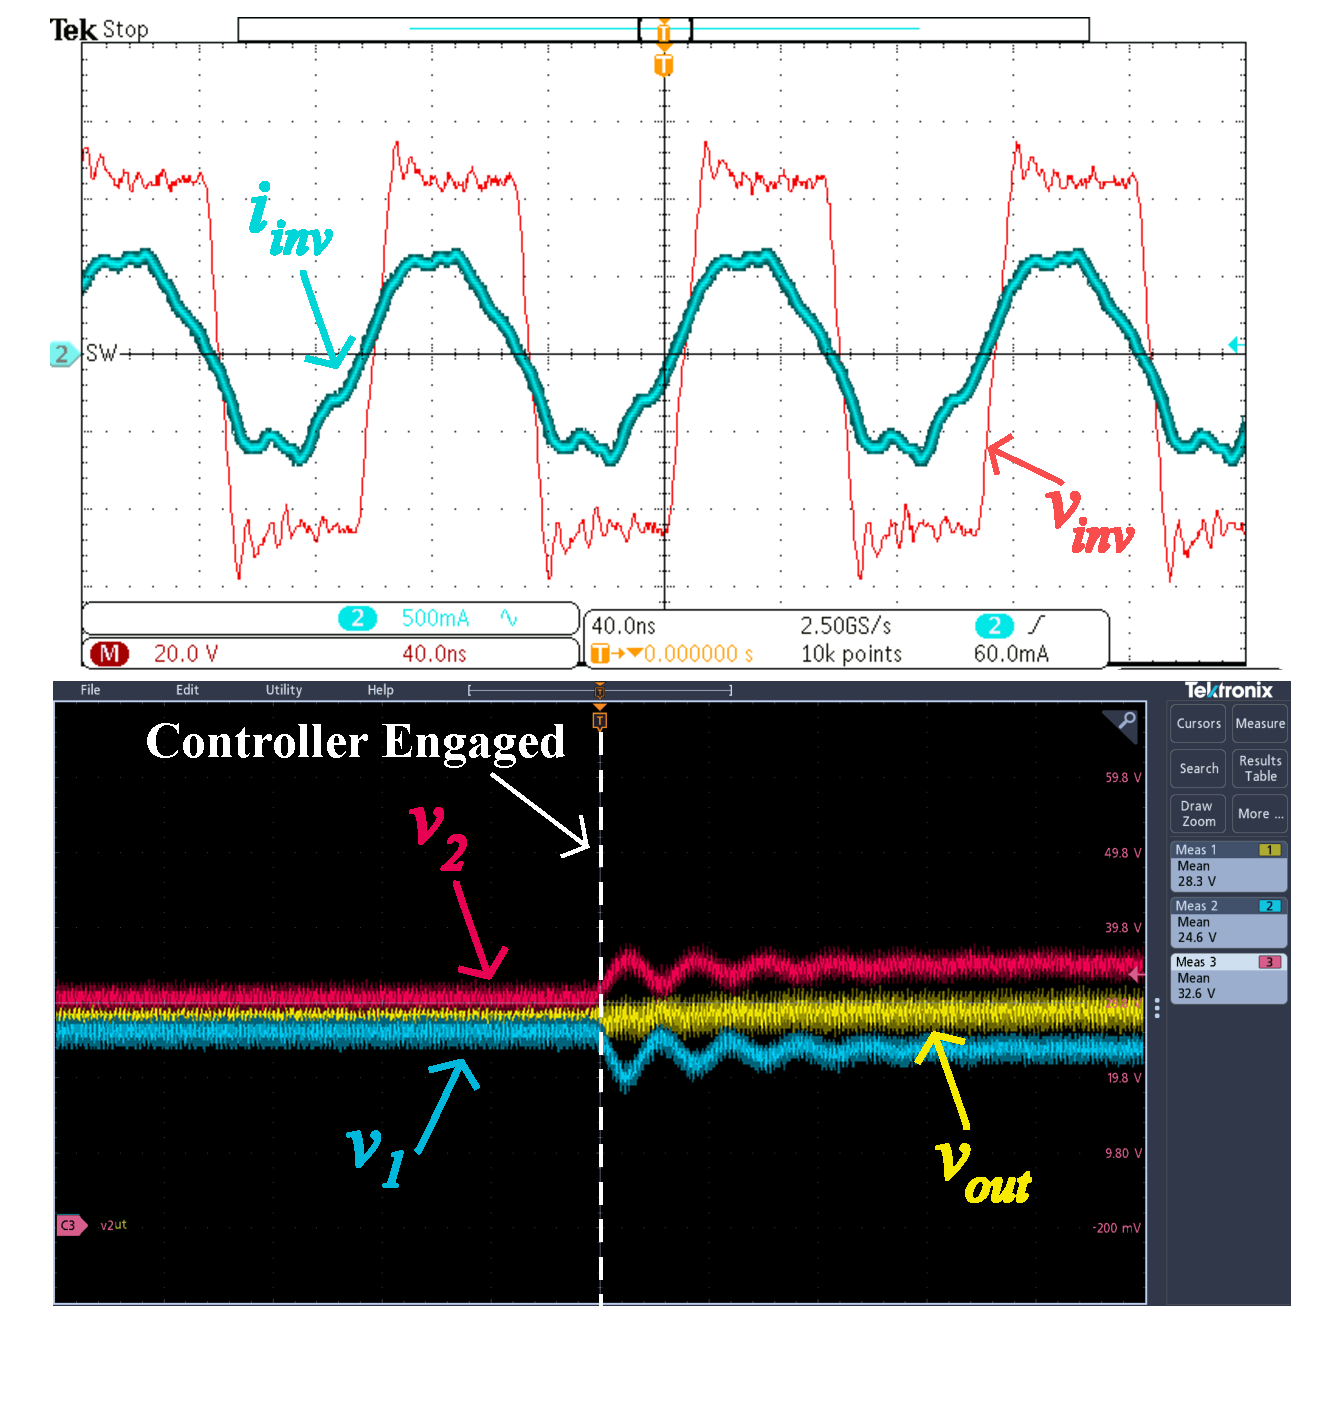
\includegraphics[width=0.7\linewidth]{figures/hardware_waveforms_annotated_eps.eps}
  \vspace{-0.4cm}
  \caption{Top: inverter switch node voltage $v_{inv}$ and current $i_{inv}$. Bottom: controller activation transient showing $v_1$, $v_2$, and $v_{out}$ trajectories.}
  \label{fig:hardware_waveforms}
\end{minipage}
\vspace{-0.4cm}
\end{figure}

\vspace{-0.5cm}
\section{Hardware Prototype and Experimental Results}
\label{sec:hardware}

The proposed controller is implemented on a prototype 6.78 MHz, 12-kW AVR-equipped scalable capacitive WPT system. To achieve this power level, three 4-kW-rated full-bridge inverters and three half-bridge rectifiers in each AVR branch ($N = M = 3$) are paralleled. Figure \ref{fig:hardware_prototype} shows the hardware prototype and experimental setup with annotations labeling important components. The system has been tested at a lower power level of 100 W, and output voltage of 30 V. Figure \ref{fig:hardware_waveforms} shows the transient behavior of the converter when the controller is activated, as well as the inverter switch node voltage $v_{inv}$ and current $i_{inv}$ in steady-state. In the inverter waveforms, note that $v_{inv}$ and $i_{inv}$ are in phase and that the inverter achieves soft switching. In the transient, note that the three voltages settle to new values after the control action is taken, and that the settling time is around 1 millisecond. Full-power results at 12 kW with improved PCBs, along with an exhaustive list of important components used will be shown in the full paper. The hardware and experimental validation of the proposed topology and controller are the third significant contribution of this digest.

\vspace{-0.25cm}

\section{Conclusion and Future Work}
\label{sec:conclusion}

\vspace{-0.25cm}

This digest presents a novel architecture for scalable dynamic capacitive WPT systems. A state-space model is developed and a full state feedback controller is designed for the proposed topology. The operation of the system is validated in simulation. Finally, a 6.78-MHz, 12-kW AVR-equipped scalable capacitive WPT system with three 4-kW-rated full bridge inverters and three half-bridge rectifiers in each AVR branch is built. Its operation is then validated in a dynamic setting.

\newpage

\footnotesize
\begin{spacing}{1.0}
\bibliographystyle{ieeetr}
\bibliography{refs}
\end{spacing}

\end{document}